\documentclass[11pt,a4paper]{article}
\usepackage[T1]{fontenc}
\usepackage{lmodern,microtype,amsmath,amssymb,booktabs,graphicx,xcolor}
\usepackage[margin=25mm,top=21mm,bottom=23mm]{geometry}
\usepackage[colorlinks=true,linkcolor=teal!55!black,citecolor=teal!55!black,urlcolor=teal!55!black]{hyperref}
\hypersetup{pdftitle={When Does a Sibling Query Preserve Necessary Access?},pdfsubject={Matched-excess evaluation of column-read policies}}
\pdfinfoomitdate=1
\pdftrailerid{}
\raggedbottom
\setlength{\parindent}{1.2em}
\setlength{\parskip}{2pt}
\setlength{\textfloatsep}{13pt}
\graphicspath{{paper/figures/}}
\newcommand{\artifact}[2]{\href{https://github.com/oraoraoraaa/least-privilege-lab/#1}{#2}}
\newcommand{\code}[1]{\texttt{#1}}
\emergencystretch=1em
\newcommand{\coveragerows}{%
JOB & 129 & 113 & 31/33 & 109 & 19 & 191/594 \\
STATS & 51 & 146 & 24/45 & 117 & 24 & 1,826/1,920 \\
}

\newcommand{\primaryrows}{%
JOB & 95\% matched & 80.0 & 90.4 & 80.9 & 10.5 & [2.0, 22.4] \\
JOB & Four grants & 66.4 & 84.3 & 66.1 & 17.9 & [6.7, 31.1] \\
STATS & 95\% matched & 7.3 & 15.0 & 7.8 & 7.7 & [1.9, 15.8] \\
STATS & Four grants & 11.3 & 16.9 & 9.5 & 5.6 & [-1.2, 13.9] \\
}

\newcommand{\sensitivityrows}{%
JOB & All informative & 19 & 191 & 80.0 & 90.4 & 10.5 \\
JOB & $H\ne D$ & 15 & 107 & 78.5 & 78.5 & 0.0 \\
JOB & Three distinct footprints & 5 & 33 & 89.3 & 89.3 & 0.0 \\
JOB & Five-neighbor ranking & 19 & 191 & 66.4 & 79.9 & 13.5 \\
JOB & Five-neighbor, distinct & 5 & 33 & 53.1 & 57.6 & 4.4 \\
STATS & All informative & 24 & 1,826 & 7.3 & 15.0 & 7.7 \\
STATS & $H\ne D$ & 24 & 1,800 & 6.9 & 13.4 & 6.5 \\
STATS & Three distinct footprints & 24 & 1,671 & 7.3 & 13.8 & 6.5 \\
STATS & Five-neighbor ranking & 24 & 1,826 & 10.8 & 15.6 & 4.8 \\
STATS & Five-neighbor, distinct & 24 & 1,671 & 10.5 & 14.2 & 3.7 \\
STATS & Join-based families & 21 & 1,132 & 3.6 & 6.6 & 3.0 \\
STATS & Join-based, distinct & 21 & 1,005 & 3.5 & 6.1 & 2.6 \\
}

\begin{document}
\begin{center}
{\LARGE\bfseries When Does a Sibling Query Preserve\\[2pt] Necessary Access?\par}
\vspace{5pt}
{\large An equal-excess evaluation of column-read policies\par}
\vspace{7pt}
{\small Research manuscript \enspace$\cdot$\enspace November 2026}
\end{center}

\begin{abstract}
A policy derived from one successful query can deny its next variant. Can preparing a related query in staging help a reviewer decide which additional columns to keep? We measured native SQLite read authorizations for 259 published SQL statements from two benchmarks. For each eligible query family we held out a third variant and compared rankings at equal numbers of retained excess grants. Among variants requiring unseen permissions, sibling evidence raised family-averaged whole-query success from 80.0\% to 90.4\% on the Join Order Benchmark (JOB) and from 7.3\% to 15.0\% on STATS-CEB. The improvement had different origins. On JOB the primary rankings tied on every one of the 107 informative comparisons where the sibling and hidden query had different read sets. After collapsing duplicate read sets in STATS, the gain was still 6.5 percentage points. Grouping STATS more narrowly by join columns reduced the gain to 3.0 points on the resulting informative cohort. A separate test fixed four additional grants before revealing the hidden query and checked 15,084 decisions with the native authorizer. On distinct STATS footprints this policy gained 4.7 points, with a family-bootstrap interval of $[-2.4,13.5]$. Reporting both exact repeats and whole-query failures changes the assessment of what one staged variant can establish.
\end{abstract}

\section{Introduction}
A reporting job can finish successfully even if it takes only one of several paths through a schema. A reviewer who removes every unused grant may break the other paths. Keeping broadly scoped grants avoids some of these denials at the cost of authority that the job never needs. The review becomes more interesting when a developer can supply a second report variant for preflight. Its read set identifies specific permissions to investigate. The next live variant can still differ from both examples.

This paper asks how much information that staged sibling contributes \emph{at the same cost in unused permissions}. Comparing a broad policy with a narrow one confounds evidence quality with permission budget. Counting individual reads correctly can also hide application failure. A query requiring six new reads fails even if the reviewer recovers five of them. We therefore compare whole statements at matched excess and repeat the comparison with a policy chosen before the hidden statement is revealed.

Two observations motivate the experiment. An exhaustive replay of published access-control data shows that an unobserved action can disappear completely from a policy derived from successful events. A constructed recovery workflow then exhibits the same failure after a scheduled drill completes. The main experiment moves to independently authored SQL programs, where staging, holding out a variant, and testing a proposed policy all have executable definitions. The contribution is a measurement of the incremental value of sibling evidence, an exact comparison for tied rankings, and an archive that lets a reader trace an aggregate result to individual permissions.

\section{What a successful run tells the reviewer}
\paragraph{A missing action.}
Restricter supplies a generated classroom snapshot, original and intended Cedar policies, and an access log~\cite{restricter}. We replayed every combination of 12 staff, two assignment actions and 13 assignments under empty context. A Java implementation of the loose course-membership rules agreed with the original Cedar engine on all 312 decisions. Deleting one membership in the Java input changed four decisions. The original policy allowed 60 tuples, of which the authors' intended policy allowed 26.

Keeping only observed authorized tuples retained 16 of those 26 even with all 26 in-scope log rows. Retaining the 13 editing rows alone kept seven intended grants and removed all 13 posting grants. Under uniform selection of 13 rows, the exact mean over $\binom{26}{13}=10{,}400{,}600$ subsets was 10.27 intended grants, including 5.54 posting grants. Repetitions in the log make rows and grants different units. An action-wide gap changes which requests survive a fixed observation budget.

\paragraph{A completed drill.}
In a controlled model-registry fixture, a service can restore from an archive or finish its drill from a warm cache. A tightening tool preserves owner-protected and observed requests. An optional rule defers tightening until a complete cycle of each associated workflow has been recorded. Across four schedules and two settings, finite enumeration and an independent Z3 encoding confirmed that all eight proposals preserved explicit requirements and granted nothing new. Before a first drill or after a logging gap, deferral preserved a later cold restore and one unnecessary old-archive grant. After a warm-cache drill, both settings denied the later cold restore. Verification proved exactly the supplied requirements. A recurring workflow can have another legitimate path that none of its observations exercised.

\paragraph{From paths to permissions.}
The SQL experiment treats the staged alternative as evidence that the reviewer can actually collect. Imagine an observed report that reads a user identifier. A second version adds a filter on a user's reputation. Preflighting that version reveals the reputation read. If the next report also filters on reputation, prioritizing that column can help. If it filters on a different column, the same choice can displace the grant that the next report needs. The experiment measures both outcomes.

\begin{figure}[htbp]
\centering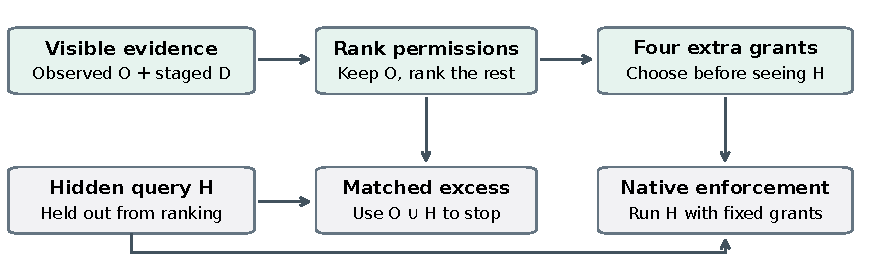
\includegraphics[width=.95\linewidth]{design.pdf}
\caption{Information available at each decision. The upper row forms policies from visible evidence and a background catalog described in Section~\ref{sec:design}. The lower row uses the hidden query twice, once to compare rankings at equal excess and once to test the independently fixed policy.}
\label{fig:design}
\end{figure}

\section{Design and measurement}\label{sec:design}
\paragraph{Permission model.}
One reporting principal initially holds the full read universe $U$ of its published schema. Each column is one resource. Each table also supplies a table-only resource for SQLite's empty-column read callback, such as a table read for a count that references no column~\cite{sqlite}. Grants cover read callbacks from projections, joins, filters and aggregates. SELECT and function callbacks are allowed uniformly. For a statement $q$, let $R(q)\subseteq U$ be the set of distinct resources requested under the full policy. Under candidate $P$, the predicted success is $\mathbf{1}\{R(q)\subseteq P\}$. This model measures access under one principal and a fixed schema. Row contents, functions outside the tested statements, writes and changes of identity require different models.

\paragraph{Workloads and folds.}
We used every published query in the Join Order Benchmark (JOB) on its movie schema~\cite{job} and all 146 statements in the STATS-CEB workload on its simplified question-and-answer schema~\cite{stats}. For JOB, filenames identify the query family. For STATS, the registered family key is the sorted set of relations in the FROM clause. This analyst-defined key supplies the experimental pairing. Family discovery in an unlabeled deployment would require a separate source of workflow information.

A fold assigns three distinct statement IDs in the same family to the roles observed, staged and hidden. Write $O,D,H$ for their permission sets. Code can differ while the sets coincide. We enumerated all ordered assignments in families with at least three IDs. The protocol's cap of 512 assignments per family was never reached. There is no chronology in the split. The finite operational contract requires the observed and hidden jobs, so its permissions are $T=O\cup H$. Reads unique to the staged job count as excess for this contract. An operator who also promises to run the staged job would choose a larger contract.

\begin{table}[htbp]\centering\small
\caption{Coverage. Eligible families have at least three distinct statement IDs. Informative folds require at least one hidden read absent from the observed variant. All 259 statements executed under the initial policy.}
\label{tab:coverage}
\begin{tabular}{@{}lrrrrrr@{}}\toprule
 & & & Eligible / all & Eligible & Informative & Informative / all\\
Corpus & $|U|$ & SQL IDs & families & IDs & families & folds\\\midrule
\coveragerows
\bottomrule\end{tabular}
\end{table}

\paragraph{Instrumentation.}
We initialized each empty schema in SQLite 3.53.1 through APSW 3.53.1.0. On STATS the loader removed the published cardinality prefix and literal timestamp casts for SQLite compatibility. Each statement was freshly prepared with caching disabled and run to completion. The native authorizer recorded each read. Empty tables suffice for the compile-time access requests of these statements. We use neither the returned counts nor a query's execution time. For enforcement we replayed the original normalized SQL, denying any read outside a candidate policy. We compared every resulting allow or denial with set containment. Unexpected operation types, unknown resources and disagreements stop the run.

\paragraph{Comparators.}
Every ranking retains $O$ and orders candidates in $U\setminus O$. \emph{Table/frequency} prioritizes columns from a table touched by $O$, then the number of query IDs in \emph{other} families that read each resource. All target-family IDs are excluded from that frequency, including the hidden ID. The \emph{sibling} ranking first prioritizes membership in $D$, then uses identical table and frequency keys. A \emph{within-table mask} substitutes a deterministic sample of columns for $D\setminus O$ with exactly the same number per table. Its seed uses only visible IDs and family. \emph{Uniform} ties all candidates. We also test literal policies $O$ and $O\cup D$. Singletons and pairs can supply background counts even when they cannot supply a target fold.

\section{Evaluating two kinds of decision}
\paragraph{Matched excess.}
Let $E=|U\setminus T|$. At our primary operating point each ranking may retain exactly $B=\lfloor 0.05E\rfloor$ excess resources. The evaluator keeps the longest prefix with at most $B$ excess resources. A useful resource immediately following the last affordable excess resource still counts. Each complete ordering therefore keeps the same number of excess resources, although retained policy sizes can differ. Integer rounding makes realized removal at least 95\%. On informative folds this allows five excess grants in JOB and one or two in STATS. The evaluator needs $H$ to locate this cutoff. It measures the quality of the ordering at a common exposure, and its success rates have the benefit of hindsight.

We integrate uniformly over tied orderings. Consider the first tier that cannot be taken in full. Let $g$ be its number of needed unseen reads, $b$ its number of excess reads, and $r<b$ the remaining excess allowance. The retained part ends just before the $(r+1)$st excess read. A particular needed read lies in one of the $b+1$ gaps around the excess reads, all equally likely, so the expected number retained from this tier is $g(r+1)/(b+1)$. When all outstanding needed reads lie in the tier, complete success requires all $g$ to occur among its first $g+r$ positions. Thus
\[
 \Pr(\text{success at the boundary})=
 \binom{g+r}{g}\bigg/\binom{g+b}{g}.
\]
Any needed read below the boundary forces failure. For example, a tied tier with two needed reads, three excess reads and one excess slot yields whole-query success $3/10$ and one needed read retained in expectation. Direct enumeration of small tied rankings checks both quantities, including cases with needed reads outside the candidate domain.

\paragraph{Fixed policy.}
The operational comparison fixes four additional grants before observing $H$. It breaks ties by the SHA-256 digest of the permission name, shared across methods. This budget was set in the protocol and held constant for both schemas. It measures one feasible policy choice and exposes the opportunity cost of promoting one column over another. For each fold we also evaluate $O$ and $O\cup D$. All six policies go through the native authorizer (Figure~\ref{fig:design}). Whole-query success requires every read. The secondary read-retention score is the fraction of $H\setminus O$ retained.

\paragraph{Unit of analysis.}
The primary cohort comprises folds with $H\setminus O\ne\varnothing$. Otherwise any candidate that preserves $O$ succeeds. We average fold scores within family, then give each informative family equal weight within its corpus. A large family contributes more ordered triples but has the same final weight as a small one. We report paired differences between methods and percentile intervals from 2,000 paired resamples of families (seed 20261120). These intervals describe sensitivity to the mix of benchmark families. Ordered triples reuse SQL statements and families share schema columns. The benchmarks have no probability-sampling design from which to infer a population of applications.

\section{Results}
\begin{table}[htbp]\centering\small
\caption{Whole-query success (\%) on informative folds. Gain is sibling minus table/frequency, in percentage points, with the family-bootstrap interval. Matched scores average over boundary ties. Four-grant scores use native enforcement.}
\label{tab:primary}
\begin{tabular}{@{}llrrrrr@{}}\toprule
Corpus & Decision & Table/freq. & Sibling & Mask & Gain & 95\% interval\\\midrule
\primaryrows
\bottomrule\end{tabular}
\end{table}

At matched excess, sibling evidence increased average success on both corpora (Table~\ref{tab:primary}). The paired JOB difference came from five improving families and 14 ties. STATS had 11 improving families, nine ties and four losses. The uniform ranking scored 4.4\% on JOB and 0.9\% on STATS. Including easy folds where $O$ already covers $H$ raised matched sibling success to 96.0\% and 18.0\%, respectively, with baselines of 93.2\% and 11.4\%. Selecting informative folds changes the question and sometimes the family denominator (Table~\ref{tab:coverage}).

\begin{figure}[htbp]
\centering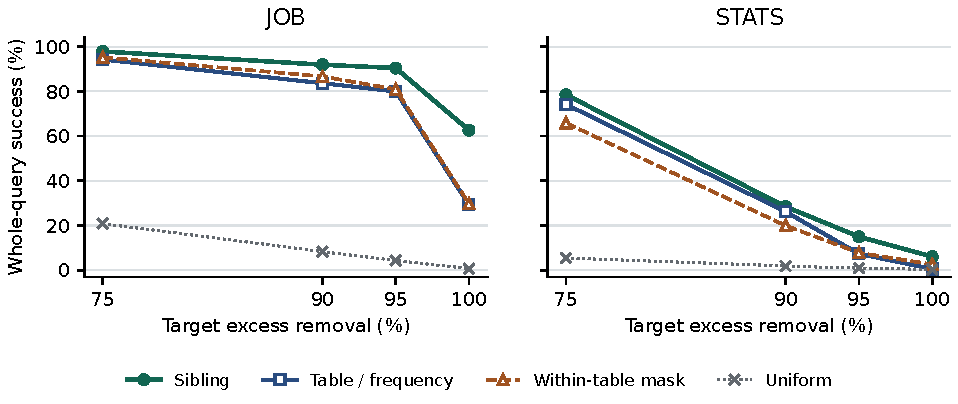
\includegraphics[width=.96\linewidth]{operating-points.pdf}
\caption{Family-averaged success at the four registered excess-removal targets. Each marker is an evaluated point. Segments connect measurements of the same ranking. Both panels use the same axes.}
\label{fig:points}
\end{figure}

The choice of exposure matters (Figure~\ref{fig:points}). On STATS, reducing target removal from 95\% to 75\% raised sibling success from 15.0\% to 78.5\%. At 95\%, sibling ranking retained 37.3\% of previously unseen reads on average, against 21.6\% for table/frequency. Whole statements succeeded much less often. Of the 1,826 informative STATS folds, 1,602 required at least two new reads. Only 32 of 191 informative JOB folds did. The number of required reads helps explain how recovering a substantial fraction of them can coexist with frequent denials.

At the four-grant budget the native engine matched the containment prediction for all $6\times 2{,}514=15{,}084$ policies and folds. Sibling ranking kept an average of 2.88 unused additions on JOB and 2.66 on STATS, compared with 3.07 and 3.04 for table/frequency. STATS's fixed-budget gain was 5.6 points, with a family-bootstrap interval spanning zero. The literal union $O\cup D$ succeeded on 52.6\% of JOB and 10.0\% of STATS informative comparisons, at different grant budgets. The observed-only policy failed on every informative fold by construction.

\section{What accounts for the difference?}
The trace archive revealed 54 repeated within-family footprints beyond their first occurrence in JOB and four in STATS. Distinct SQL IDs therefore do not establish that the staged variant requires a different set of permissions from the hidden variant. We recorded a post-result audit before conducting the checks below. The primary comparison and operating points were fixed earlier.

\begin{table}[htbp]\centering\small
\caption{Post-result checks at 95\% targeted removal on informative folds. Rates are whole-query success percentages. Blind is the comparator without $D$. The five-neighbor rows change the baseline. The join-based rows also change the eligible cohort and background counts.}
\label{tab:audit}
\begin{tabular}{@{}llrrrrr@{}}\toprule
Corpus & Cohort or comparison & Families & Folds & Blind & Sibling & Gain (pp)\\\midrule
\sensitivityrows
\bottomrule\end{tabular}
\end{table}

\paragraph{Exact reuse and transfer.}
Removing folds where $H=D$ left 107 informative JOB assignments. The primary two rankings tied \emph{on every one}. We then collapsed each family's identical footprints to its first SQL ID before forming triples. Just five JOB families could still supply three distinct footprints, and both rankings scored 89.3\% there. On STATS, 24 families survived, and the sibling gain remained 6.5 points (Table~\ref{tab:audit}). The higher JOB absolute success after collapsing reflects a different family mix. Under the fixed four-grant policy on distinct footprints, JOB instead scored 68.7\% versus 54.0\% (five families). STATS scored 15.9\% versus 11.2\%, a gain of 4.7 points with interval $[-2.4,13.5]$. The JOB tie therefore applies specifically to the primary matched comparison.

\paragraph{Would another source of column evidence do as well?}
Across 32 additional reproducible within-table masks, primary success ranged from 76.2\% to 81.7\% on JOB and from 6.3\% to 11.0\% on STATS. Promoting the single most similar outside-family query to $O$ (Jaccard similarity of read sets, ties by query ID) gave 63.3\% and 8.3\%. These results separate specific evidence from the mere act of promoting columns. A second baseline ranked candidates by frequency among the five closest outside-family statements, including all ties at fifth place, then by the original keys. On STATS it raised blind success to 10.8\% and narrowed the sibling gain to 4.8 points. On distinct JOB footprints the alternative ranking gained 4.4 points from $D$ but reached only 57.6\%, below both primary rankings. Incremental value depends on the baseline even when absolute policy quality declines.

\paragraph{Which families and which universe?}
Requiring equal sets of joined column pairs in addition to equal tables split STATS into 58 groups. Ninety-two statements remained eligible. The paired gain shrank to 3.0 points across 21 informative families and 2.6 after footprint collapse. Both the prediction problem and its case mix change under this regrouping. A separate registered check restricted $U$ to tables touched by $O$ or $D$ and charged any hidden read beyond them as a miss. Sibling versus baseline then scored 77.9\% versus 53.2\% on JOB and 6.6\% versus 0.6\% on STATS. Shrinking the initial universe also shrinks its allowable count of excess grants. Using only permissions exercised by $O$, $D$, or other-family statements gave 84.0\% versus 62.3\% on JOB and 11.5\% versus 5.0\% on STATS.

\paragraph{Two native decisions.}
Under the four-grant policy, JOB variant \code{10c} was observed, \code{10a} staged, and \code{10b} held out. The missing read was \code{role\_type.role}. Both policies added the same three other columns. Sibling evidence used the fourth slot on the required read, while table/frequency spent it on \code{title.kind\_id}. The engine admitted the sibling policy's query. In STATS the direction reversed. After observing \code{q039} and staging \code{q038}, the hidden query \code{q116} needed \code{users.views}. The staged query promoted \code{badges.date} into that slot. Table/frequency admitted the hidden query and the sibling policy denied it. The archive identifies these triples and lists every proposed addition.

\section{Interpretation and related work}
\paragraph{What the measurements establish.}
The staged variant is most useful when it contains information about the hidden variant that is absent from both the observation and the background ranking. On JOB, separating exact reuse from transfer removes the entire primary gain. The de-duplicated STATS comparison supplies evidence for transfer across different read sets. Its absolute success of 13.8\% also quantifies the residual risk of using this ranker as a policy selector. Even hindsight about the allowable cutoff left most complete hidden queries uncovered at the specified exposure. An operator promising a critical report can preflight its known paths and protect their observed reads explicitly. The experiments give little basis for treating one passing sibling as certification for other variants.

\paragraph{Policy mining and tightening.}
Cotrini, Weghorn and Basin study learning attribute-based rules from sparse logs and the difficulty of treating unobserved requests as negative examples~\cite{rhapsody}. IAM-PolicyRefiner narrows existing AWS policies and evaluates exercise of held-out requests~\cite{iam}. Restricter synthesizes tighter Cedar rules subject to log and semantic constraints~\cite{restricter}. OPMonitor examines excess permissions that survive policy verification~\cite{monitor}. Our classroom case reuses public Restricter inputs to calibrate missing observations. The ensuing rankings compare finite read grants under a common exposure budget. Holding exposure constant lets us ask how much a separate preflight contributes to availability of an entire held-out job.

\paragraph{Least privilege for database programs.}
ShillDB gives programs constrained database capabilities and uses contracts to express permissible access~\cite{shilldb}. SQLite's authorizer supplies the native read-level enforcement point in this study~\cite{sqlite}. These mechanisms make the requirements of a known statement enforceable. Predicting resources for a different statement requires outside evidence. JOB and STATS were designed to evaluate optimizers and cardinality estimators~\cite{job,stats}. Their reusable query variants make the prediction test executable and also create the template repetition that our audit measures.

\paragraph{Scope and next experiment.}
Our contract contains two jobs, every grant has unit cost, and the initial policy covers the schema. A real service may need a staged job permanently, may assign more risk to one column than another, or may start from a much narrower policy. Expanding the intended contract would relabel some of the measured excess as required. Two public query workloads and a constructed recovery fixture provide executable cases. Production incidence requires representative service histories. The measured outcome is authorization of a statement on an empty schema. End-to-end availability would also require validating returned data, other application steps and their permissions.

A direct external test would freeze candidates from one release of a reporting application, preflight alternatives identified by its maintainers using only that release, and score every query exercised in a later release. The denominator would include jobs for which no sibling was available. Recording exact-footprint repeats separately would show whether the effect comes from reuse, genuine transfer, or both. That experiment would answer a prospective deployment question that retrospective triples cannot settle.

\section{Conclusion}
A sibling preflight can improve the ordering of permissions at a fixed exposure, but a high aggregate score can conceal where the information came from. In one benchmark the entire registered advantage arose when distinct SQL statements requested identical permissions. In another, the advantage persisted across distinct footprints and shrank under a stricter definition of relatedness. Evaluations of least-privilege policies should report whole-job success, the number of unused permissions retained, and performance after exact footprint reuse is removed. Together these measurements distinguish a rehearsed execution from evidence about the next one.

\clearpage
\section*{Artifact and research provenance}
The \artifact{tree/305bd2bbcc84a3e3fa690c72cd6253d148928f16/research/paths}{experiment archive} includes pinned source inputs by reference and digest, the \artifact{blob/305bd2bbcc84a3e3fa690c72cd6253d148928f16/research/paths/PROTOCOL.md}{pre-measurement protocol}, the \artifact{blob/305bd2bbcc84a3e3fa690c72cd6253d148928f16/research/paths/AUDIT.md}{post-result audit plan}, all statement footprints, fold identities, policy outcomes and aggregation code. The classroom and registry studies have separate inputs, protocols and checks. From the research branch, \code{sh research/reproduce.sh} regenerates all three studies. Fresh checkouts on macOS arm64 and Arch Linux x86-64 reproduced the archived measurement contents. \code{make paper} rebuilds the figures, tables and PDF. Codex designed and executed this branch's experiments, analyzed the results and drafted this manuscript at the repository owner's request. No production credentials, customer records or human-subject data were collected for the experiments.

\begin{thebibliography}{9}\small
\bibitem{rhapsody} C. Cotrini, T. Weghorn, and D. Basin. Mining ABAC Rules from Sparse Logs. \emph{IEEE European Symposium on Security and Privacy}, 2018. \href{https://people.inf.ethz.ch/~basin/pubs/eurosnp18.pdf}{Author copy}.
\bibitem{iam} L. D'Antoni, S. Ding, A. Goel, M. Ramesh, N. Rungta, and C. Sung. Automatically Reducing Privilege for Access Control Policies. \emph{Proceedings of the ACM on Programming Languages}, OOPSLA, 2024. \href{https://doi.org/10.1145/3689738}{doi:10.1145/3689738}.
\bibitem{restricter} K. L. Wu, C. Jenkins, S. D. Stoller, and O. Chowdhury. Automatically Tightening Access Control Policies with Restricter. \emph{TACAS}, 2026. \href{https://doi.org/10.1007/978-3-032-22752-2_6}{Publisher record}.
\bibitem{monitor} X. Wang, Y. Guo, Z. Sun, M. Yu, F. Li, and L. Fang. OPMonitor: Continuously monitoring residual over-granted permissions in verified access control policies. \emph{Computers \& Security}, 158, 104623, 2025. \href{https://doi.org/10.1016/j.cose.2025.104623}{Publisher record}.
\bibitem{shilldb} E. Zigmond, S. Chong, C. Dimoulas, and S. Moore. Fine-Grained, Language-Based Access Control for Database-Backed Applications. \emph{The Art, Science, and Engineering of Programming}, 4(2), 2020. \href{https://people.seas.harvard.edu/~chong/abstracts/ZigmondCDM2020.html}{Author copy}.
\bibitem{job} V. Leis, A. Gubichev, A. Mirchev, P. Boncz, A. Kemper, and T. Neumann. How Good Are Query Optimizers, Really? \emph{Proceedings of the VLDB Endowment}, 9(3), 2015. \href{https://www.vldb.org/pvldb/vol9/p204-leis.pdf}{Paper}.
\bibitem{stats} Y. Han et al. Cardinality Estimation in DBMS: A Comprehensive Benchmark Evaluation. \emph{Proceedings of the VLDB Endowment}, 15(4), 752--765. \href{https://doi.org/10.14778/3503585.3503586}{doi:10.14778/3503585.3503586}, 2021.
\bibitem{sqlite} SQLite. Compile-Time Authorization Callbacks. \emph{SQLite C Interface}. \href{https://www.sqlite.org/c3ref/set_authorizer.html}{API reference}.
\end{thebibliography}
\end{document}
